% Compile with XeLaTeX.
\documentclass[12pt,a4paper]{article}

\usepackage{fontspec}
\setmainfont{Times New Roman}
\usepackage{polyglossia}
\setmainlanguage{vietnamese}
\usepackage[a4paper,margin=2.5cm]{geometry}
\usepackage{graphicx}
\usepackage{booktabs}
\usepackage{longtable}
\usepackage{array}
\usepackage{enumitem}
\usepackage{hyperref}
\usepackage{xcolor}
\usepackage[most]{tcolorbox}
\usepackage{titlesec}

\graphicspath{{../figures/}{figures/}}
\hypersetup{
    colorlinks=true,
    linkcolor=black,
    urlcolor=blue
}

\definecolor{boxblue}{HTML}{EAF2FF}
\definecolor{boxborder}{HTML}{2F5597}
\setlist[itemize]{leftmargin=1.2cm,itemsep=0.2em}
\setlist[enumerate]{leftmargin=1.2cm,itemsep=0.2em}
\titleformat{\section}{\Large\bfseries}{\thesection.}{0.6em}{}
\titleformat{\subsection}{\large\bfseries}{\thesubsection.}{0.6em}{}

\newcommand{\placeholder}[1]{\textbf{[#1]}}

\begin{document}

\begin{titlepage}
    \centering
    \vspace*{1cm}
    {\Large \placeholder{Tên trường}\par}
    \vspace{0.4cm}
    {\large \placeholder{Khoa / Bộ môn}\par}
    \vspace{1.5cm}
    {\Huge\bfseries Báo cáo dự án\par}
    \vspace{0.4cm}
    {\LARGE\bfseries Energy Theft Detection using Machine Learning\par}
    \vspace{1.5cm}

    \begin{tcolorbox}[colback=boxblue,colframe=boxborder,width=0.88\textwidth,arc=2mm]
        \begin{tabular}{@{}p{0.36\textwidth}p{0.46\textwidth}@{}}
            Môn học & \placeholder{Tên môn học} \\
            Giảng viên & \placeholder{Tên giảng viên} \\
            Số thứ tự nhóm & \placeholder{Số thứ tự nhóm} \\
            Tên nhóm & \placeholder{Tên nhóm} \\
            Nhóm trưởng & \placeholder{Họ tên nhóm trưởng} \\
            Thành viên & \placeholder{Danh sách thành viên} \\
            Link GitHub & \placeholder{URL repository GitHub} \\
        \end{tabular}
    \end{tcolorbox}

    \vfill
    {\large \placeholder{Thành phố}, \placeholder{Tháng/Năm}\par}
\end{titlepage}

\tableofcontents
\newpage

\section{Tóm tắt}

Dự án xây dựng pipeline học máy để phát hiện khách hàng có khả năng trộm điện từ dữ liệu tiêu thụ điện hằng ngày. Bộ dữ liệu có 42,372 khách hàng, nhãn nhị phân \texttt{FLAG}, và 1,034 cột ngày tiêu thụ. Do tỷ lệ khách hàng theft chỉ khoảng 8.53\%, bài toán có mất cân bằng lớp rõ rệt. Vì vậy, báo cáo ưu tiên các chỉ số Recall, F2, PR-AUC, ROC-AUC và confusion matrix thay vì chỉ dùng Accuracy.

\begin{tcolorbox}[colback=boxblue,colframe=boxborder,title=Kết quả chính,arc=2mm]
Mô hình tốt nhất hiện tại là LightGBM benchmark với F2 = 0.5176, Recall = 0.6458, PR-AUC = 0.4489 và ROC-AUC = 0.8387 trên tập test. Logistic Regression + L2 + balanced được giữ làm baseline dễ giải thích, còn Random Forest bổ sung hướng so sánh thuộc nhóm bagging.
\end{tcolorbox}

\section{Mục tiêu và phạm vi}

Mục tiêu của dự án là xây dựng một quy trình end-to-end gồm tiền xử lý dữ liệu, tạo đặc trưng, huấn luyện mô hình, chọn ngưỡng dự đoán và đánh giá cuối trên tập test. Kết quả mô hình được hiểu như công cụ hỗ trợ sàng lọc khách hàng rủi ro cao, không phải kết luận vi phạm cuối cùng.

Phạm vi repo hiện tại gồm:
\begin{itemize}
    \item Tiền xử lý dữ liệu bằng \texttt{src/preprocessing\_v2.py}.
    \item Tạo bảng đặc trưng bằng \texttt{src/feature.py}.
    \item Huấn luyện và lưu mô hình bằng \texttt{src/train.py}.
    \item Notebook phân tích chính tại \texttt{notebooks/model\_training-codex.ipynb}.
    \item Các hình minh họa trong thư mục \texttt{figures/}.
\end{itemize}

\section{Dữ liệu}

Dữ liệu sử dụng là SGCC Electricity Theft Detection Dataset. Mỗi dòng tương ứng một khách hàng, gồm mã khách hàng \texttt{CONS\_NO}, nhãn \texttt{FLAG}, và chuỗi tiêu thụ điện hằng ngày trong giai đoạn từ 01/01/2014 đến 31/10/2016.

\begin{table}[h]
\centering
\caption{Tổng quan dữ liệu}
\begin{tabular}{lr}
\toprule
Thuộc tính & Giá trị \\
\midrule
Số khách hàng & 42,372 \\
Số cột ngày tiêu thụ & 1,034 \\
Normal customers & 38,757 (91.47\%) \\
Theft customers & 3,615 (8.53\%) \\
Tỷ lệ lệch lớp & 10.72 : 1 \\
\bottomrule
\end{tabular}
\end{table}

\section{Khám phá dữ liệu}

EDA cho thấy dữ liệu có ba đặc điểm quan trọng. Thứ nhất, phân phối tiêu thụ điện lệch phải mạnh, mean cao hơn median và có outlier rất lớn. Thứ hai, missing values chiếm khoảng 25.64\% toàn bộ ô tiêu thụ, trong đó nhóm theft có missing rate trung bình cao hơn nhóm normal. Thứ ba, các tín hiệu như zero consumption, outlier và thay đổi tiêu thụ theo thời gian khác nhau giữa hai nhóm nhãn.

\begin{figure}[h]
    \centering
    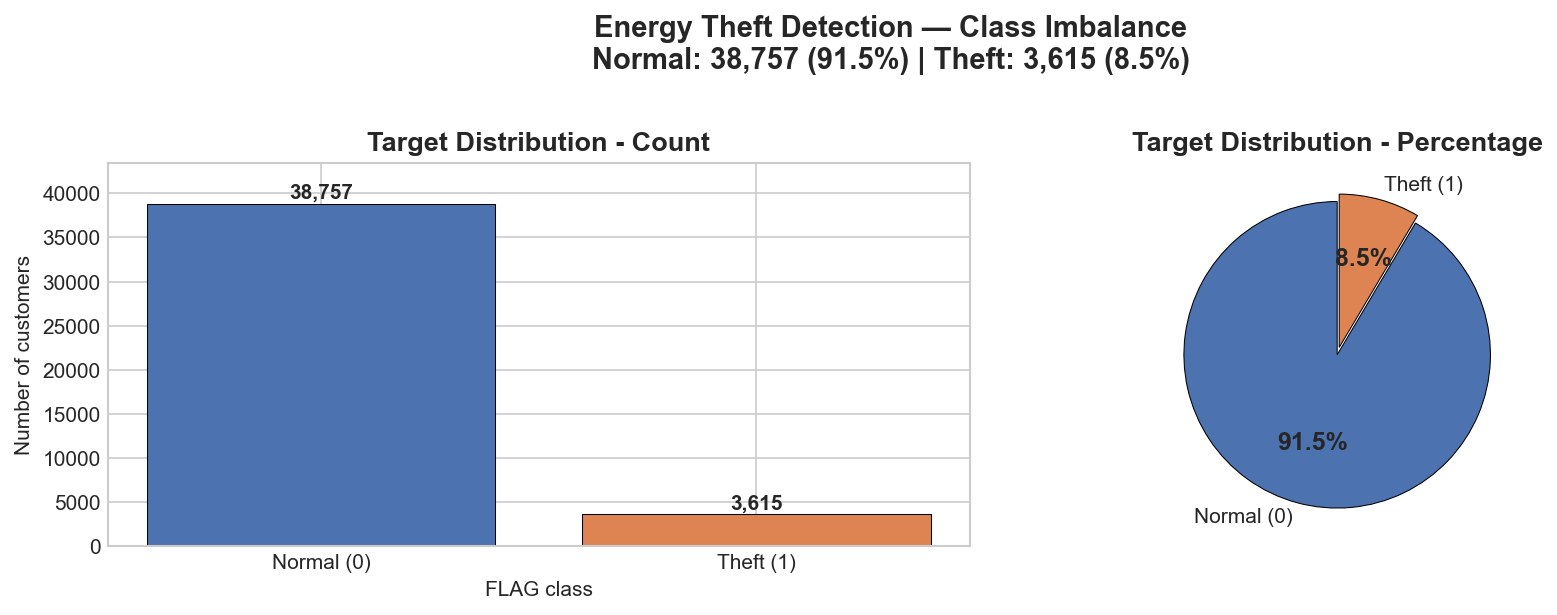
\includegraphics[width=0.68\textwidth]{01_target_distribution.png}
    \caption{Phân phối nhãn cho thấy bài toán bị mất cân bằng lớp.}
\end{figure}

Những quan sát này dẫn đến hai quyết định chính: không đánh giá mô hình bằng Accuracy đơn lẻ, và không xóa toàn bộ tín hiệu chất lượng dữ liệu vì missing/zero/outlier có thể mang thông tin hành vi.

\section{Tiền xử lý dữ liệu}

Pipeline tiền xử lý chính nằm trong \texttt{src/preprocessing\_v2.py}. Mục tiêu là làm sạch chuỗi tiêu thụ điện nhưng không tạo target leakage.

Các bước chính:
\begin{enumerate}
    \item Chuẩn hóa cột định danh, nhãn và cột ngày tiêu thụ.
    \item Tạo \texttt{quality\_features.csv} trước khi làm sạch để giữ tín hiệu missing, zero, outlier và streak.
    \item Xử lý giá trị âm bằng cách chuyển thành missing nếu có.
    \item Clip outlier lớn hơn 500 kWh/day.
    \item Fill missing theo từng khách hàng bằng forward fill, backward fill, median cá nhân và fallback global median.
    \item Kiểm tra output không còn missing, giá trị âm hoặc giá trị vượt ngưỡng clip.
\end{enumerate}

Điểm quan trọng là pipeline không dùng \texttt{FLAG} trong quá trình fill missing. Điều này giúp kết quả đánh giá sau train/test phản ánh đúng khả năng tổng quát hóa.

\section{Feature Engineering}

Feature engineering chuyển chuỗi 1,034 ngày tiêu thụ thành bảng đặc trưng cấp khách hàng tại \texttt{data/processed/features.csv}. Bảng này có 42,372 dòng và 163 cột, gồm \texttt{CONS\_NO}, \texttt{FLAG}, và 161 feature. Khi huấn luyện, hai feature hằng \texttt{negative\_count\_raw} và \texttt{negative\_ratio\_raw} được bỏ, còn 159 feature được dùng.

Các nhóm feature chính gồm:
\begin{itemize}
    \item \textbf{Thống kê tiêu thụ}: mean, median, standard deviation, quantile, IQR, range.
    \item \textbf{Zero và low consumption}: zero ratio, low ratio, max zero streak.
    \item \textbf{Xu hướng thời gian}: first/recent windows, first half vs second half, trend slope.
    \item \textbf{Biến động}: daily change, spike/drop count, spike/drop streak.
    \item \textbf{Monthly, rolling, segment, calendar}: thống kê theo tháng, rolling windows, 4 đoạn thời gian, weekday/weekend.
    \item \textbf{Quality và interaction}: missing, zero, outlier raw signals và các tương tác giữa chúng.
\end{itemize}

\section{Thiết lập huấn luyện}

Dữ liệu được chia stratified thành train, validation và test theo tỷ lệ 70/15/15. Tập validation dùng để chọn threshold, còn tập test chỉ dùng cho đánh giá cuối.

\begin{table}[h]
\centering
\caption{Chia dữ liệu}
\begin{tabular}{lrr}
\toprule
Tập dữ liệu & Số khách hàng & Theft ratio \\
\midrule
Train & 29,660 & 8.53\% \\
Validation & 6,356 & 8.54\% \\
Test & 6,356 & 8.53\% \\
\bottomrule
\end{tabular}
\end{table}

Ba mô hình được so sánh:
\begin{itemize}
    \item \textbf{Logistic Regression + L2 + balanced}: baseline tuyến tính, dễ giải thích; L2 giúp ổn định hệ số, class weight balanced giúp chú ý hơn đến lớp theft.
    \item \textbf{Random Forest}: mô hình bagging dùng nhiều cây quyết định để giảm variance.
    \item \textbf{LightGBM}: mô hình boosting phù hợp dữ liệu tabular, có khả năng học quan hệ phi tuyến và tương tác feature.
\end{itemize}

\section{Chiến lược chọn threshold}

Mỗi mô hình tạo ra score cho lớp theft. Threshold quyết định khách hàng được gán nhãn suspected theft khi score vượt ngưỡng. Với dữ liệu mất cân bằng, threshold 0.5 không nhất thiết phù hợp. Dự án chọn threshold trên tập validation theo Best F2 vì F2 ưu tiên Recall hơn Precision.

\begin{figure}[h]
    \centering
    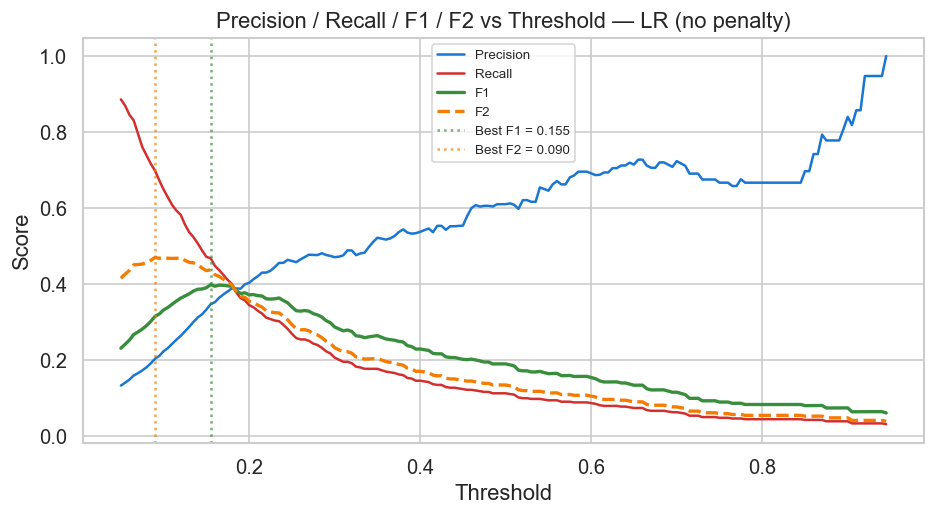
\includegraphics[width=0.78\textwidth]{threshold_tradeoff.png}
    \caption{Trade-off giữa Precision, Recall và F2 khi thay đổi threshold.}
\end{figure}

\section{Kết quả thực nghiệm}

\begin{table}[h]
\centering
\caption{Kết quả trên tập test với threshold Best F2 từ validation}
\begin{tabular}{lrrrrrr}
\toprule
Model & Threshold & Precision & Recall & F2 & PR-AUC & ROC-AUC \\
\midrule
LightGBM benchmark & 0.4368 & 0.2885 & 0.6458 & 0.5176 & 0.4489 & 0.8387 \\
Random Forest benchmark & 0.3000 & 0.2498 & 0.6439 & 0.4895 & 0.3661 & 0.8092 \\
LR + L2 + balanced & 0.5400 & 0.2162 & 0.5756 & 0.4320 & 0.3117 & 0.7772 \\
\bottomrule
\end{tabular}
\end{table}

LightGBM đạt kết quả tốt nhất trên F2, PR-AUC và ROC-AUC. Random Forest có Recall gần LightGBM nhưng Precision và PR-AUC thấp hơn, nghĩa là khả năng xếp hạng khách hàng theft kém hơn. Logistic Regression có kết quả thấp hơn nhưng vẫn hữu ích để giải thích baseline tuyến tính.

\section{Phân tích lỗi và diễn giải}

Với LightGBM tại threshold 0.4368 trên tập test:
\begin{itemize}
    \item True Positive: 350.
    \item False Negative: 192.
    \item False Positive: 863.
    \item Recall: 64.58\%.
    \item Precision: 28.85\%.
\end{itemize}

\begin{figure}[h]
    \centering
    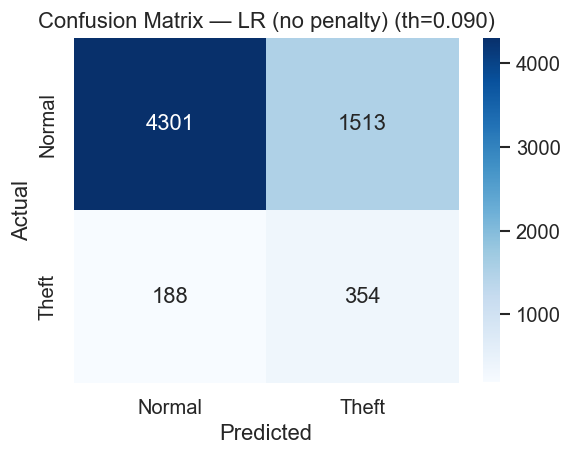
\includegraphics[width=0.62\textwidth]{confusion_matrix_test.png}
    \caption{Confusion matrix của mô hình LightGBM trên tập test.}
\end{figure}

Precision thấp là hệ quả thường gặp trong bài toán lớp hiếm. Trong bối cảnh thực tế, model nên được xem như công cụ sàng lọc: đưa ra danh sách khách hàng rủi ro cao để kiểm tra thêm, không thay thế quy trình xác minh nghiệp vụ.

\section{Lưu mô hình và khả năng demo}

Script \texttt{src/train.py} huấn luyện lại ba mô hình, chọn mô hình tốt nhất theo F2 trên test comparison, và lưu artifact trong thư mục \texttt{models/}. Artifact chính là \texttt{models/energy\_theft\_model\_bundle.pkl}, chứa model tốt nhất, threshold, danh sách feature đang dùng và metadata cần cho inference.

Web demo đề xuất nên dùng dữ liệu mẫu từ 15\% test set. Người dùng chọn một khách hàng, web hiển thị theft score, threshold, nhãn dự đoán và một số feature nổi bật. Ground truth chỉ nên bật trong chế độ học tập để so sánh, không được xem là input của model.

\section{Hướng dẫn tái lập}

Các bước tái lập kết quả trong repo:

\begin{enumerate}
    \item Cài đặt dependencies từ \texttt{requirements.txt}.
    \item Chạy preprocessing để tạo \texttt{cleaned.csv} và \texttt{quality\_features.csv}.
    \item Chạy feature engineering để tạo \texttt{features.csv}.
    \item Chạy \texttt{python src/train.py} để huấn luyện và lưu model.
\end{enumerate}

Các file đầu ra chính:
\begin{itemize}
    \item \texttt{models/energy\_theft\_model\_bundle.pkl}
    \item \texttt{models/model\_metadata.json}
    \item \texttt{models/training\_summary.csv}
    \item \texttt{models/test\_comparison.csv}
    \item \texttt{models/threshold\_report.csv}
\end{itemize}

\section{Kết luận}

Dự án đã xây dựng được pipeline hoàn chỉnh cho bài toán phát hiện trộm điện: làm sạch dữ liệu có kiểm soát, giữ lại tín hiệu chất lượng dữ liệu, tạo đặc trưng cấp khách hàng, so sánh ba mô hình đại diện cho baseline tuyến tính, bagging và boosting, sau đó chọn threshold bằng validation set.

Kết quả cuối cho thấy LightGBM là lựa chọn phù hợp nhất trong repo hiện tại. Mô hình đạt Recall 64.58\% và F2 0.5176 trên test, tốt hơn Random Forest và Logistic Regression. Tuy vậy, do precision còn thấp, hệ thống nên được dùng như công cụ hỗ trợ ưu tiên kiểm tra thay vì kết luận tự động.

\end{document}
